% !TeX root = ../skript.tex
% !TeX spellcheck = de_DE


\section{Lorenz-Modell}\label{lorenz-modell}
Die Gleichungen, welche das Lorenz-Modell beschreiben, enthalten viele physikalische Eigenschaften wie die Dichte, Geschwindigkeit und Temperatur der Atmosphäre. Lorenz wollte aus den bereits existierenden Gleichungen der Hydrodynamik ein Modell zur Wetterprognose erstellen. Basierend auf vorgehenden Werken von Saltzman startete Lorenz mit den hyrodynamischen Gleichungen und verfolgte ein systematisches Näherungsvorgehen, womit er auf die folgenden drei Gleichungen stoss:

\begin{align}
\dot{x} &= \sigma(x - y)\\
\dot{y} &= x(\rho - z) - y\\
\dot{z} &= xy - \beta z
\end{align}

Die X-Achse entspricht dabei der hydrodynamischen, räumlichen Durchschnittsgeschwindigkeit, also die durchschnittliche Windgeschwindigkeit. Die Y-Achse repräsentiert die Temperatur und die Z-Achse der Temperaturgradient. Also wie schnell sich die Temperatur verändert. 

Wie aus den obigen Gleichungen ersichtlich ist, sind drei Parameter vorhanden. Alle sind immer positiv.

\subsubsection{1. Parameter: $\sigma$}
$\sigma$ entspricht der dimensionslosen Prandtl Zahl. Diese ist das Verhältnis von \textit{Viskosität} und der \textit{Wärmeleitfähigkeit}. Da beide Eigenschaften die Einheit $\frac{\text{m}^2}{\text{s}}$ haben, resultiert daraus eine dimensionslose Zahl.

\subsubsection{2. Parameter: $\rho$}
Dieser Parameter ist nach dem Physiker Baron Rayleigh benannt worden und heisst Rayleigh Zahl. Es entspricht dem Verhältnis von \textit{Wärmeausdehnung} und der \textit{Viskosität}.

\subsubsection{3. Parameter: $\beta$}
Das $ \beta $ entspricht der \textit{Wärmeausdehnung}. Dabei handelt es sich um die Veränderung der geometrischen Abmessungen(Länge, Flächeninhalt und Volumen) eines Körpers, die sich mit erhöhter Temperatur vergrössern.

\begin{figure}
	\centering
	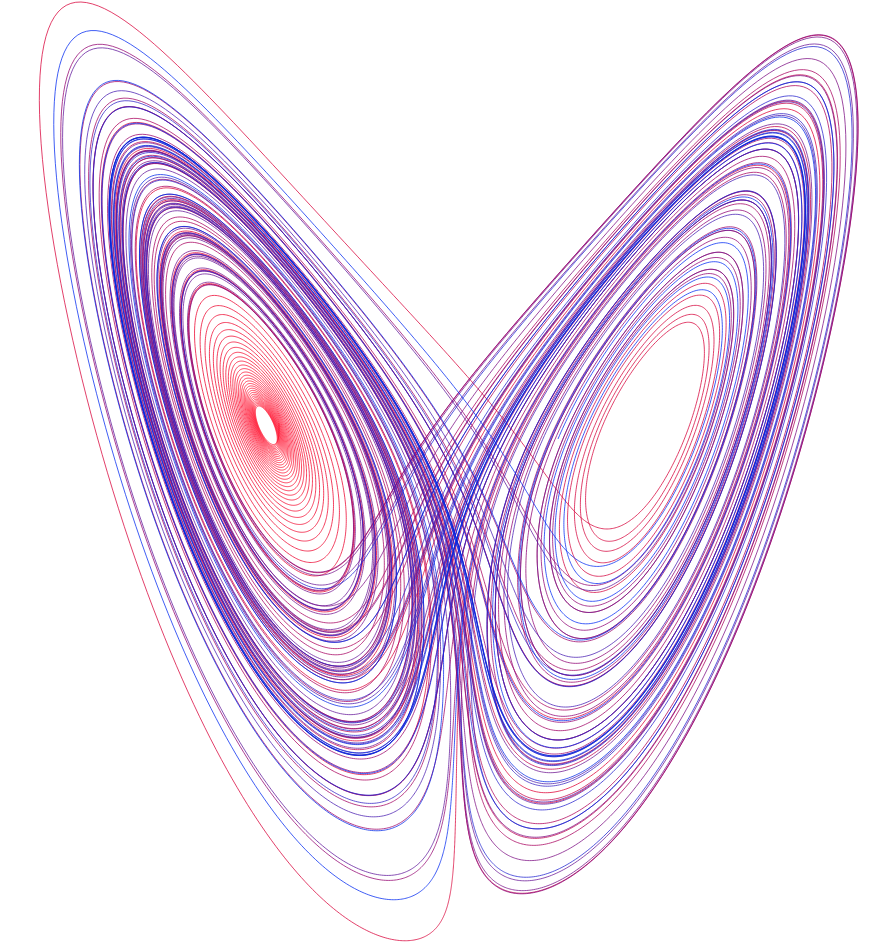
\includegraphics[width=0.3\linewidth]{lorenz/assets/lorenz-modell/lorenz-modell}
	\caption{Bahn des Lorenz-Modell mit $\rho = 28$, $\sigma = 10$ und $\beta = \frac{8}{3}$}
	\label{fig:lorenz-modell}
\end{figure}


\subsection{Numerische Lösungen}
Es gibt für das Lösen von Differentialgleichungen zwei Ansätze. Zum einen der analytische Ansatz, der eine allgmeingültige Lösung sucht. Es handelt sich bei den drei Lorenz-Gleichungen um nicht-lineare Differentialgleichungen, welche analytisch nicht lösbar sind. Aus diesem Grund fällt dieser Lösungsweg weg. 

Der zweite Ansatz ist, eine Diskretisierung vorzunehmen und den Computer für jeden definierten Zeitpunkt die Resultate der Gleichungen ausrechnen zu lassen. Dies ist auch der in dieser Arbeit gewählte Weg, der im Folgenden bis zur tatsächlichen Visualisierung genauer beschrieben wird. 

\subsubsection{Euler-Verfahren}

Wir wählten für die Diskretisierung das \textit{Einschritt-Verfahren} zur Annäherung der Werte des Lorenz-Modells. Das resultierende Gleichungssystem besteht aus einfachen Arithmetik-Operationen und ist für den Computer einfach berechenbar. Diese Effizienz erlaubt auch Smartphones die Visualisierung effizient zu berechnen und flüssig anzuzeigen.

Als Basis für dieses Verfahren nahm Euler die lineare Gleichung $ y = a \cdot x + b $. Er setzte das Ergebnis der Differentialgleichung als Steigung $ a $ ein. $x$ wird mit dem Diskretisierungsschritt belegt. Der Diskretisierungsschritt beschreibt den Abstand zweier numerischen Messungen in der Visualisierung. Anders ausgedrückt kontrolliert der Diskretisierungsschritt die Zeit, die zwischen zwei Messungen des Modells vergangen ist. Wenn dieser Schritt erhöht wird, dann nimmt der Detailgrad ab, dafür kann eine längere Zeit mit der gleichen Anzahl Messungen das Modell durch die Software aufgezeichnet werden.

Der \textit{Y-Achsenabschnitt} des linearen Gleichungssystems $ b $ wird mit dem Ergebnis der vorherigen Rechnungsschritt $ x(t) $ belegt, da der Differentialterm den Abstand vom Wert vorher berechnet.

\begin{align}
    x(t+ \Delta t) = x(t) + \frac{dx}{dt} \cdot \Delta t\\
    y(t + \Delta t) = y(t) + \frac{dy}{dt} \cdot \Delta t\\
    z(t + \Delta t) = z(t) + \frac{dz}{dt} \cdot \Delta t
\end{align}

Wir können nun die Gleichungen des Lorenz-Modells einsetzen. Dadurch entstehen die folgenden einfachen Gleichungen mit nur arithmetischen Operationen.

\begin{align}
    x(t + \Delta t) = x(t) + \sigma(x - y) \cdot \Delta t\\
    y(t + \Delta t) = y(t) + x(\rho - z) - y \cdot \Delta t\\
    z(t + \Delta t) = z(t) + xy - \beta z \cdot \Delta t
\end{align}

Dieses System entspricht dem Code der Visualisierung unterhalb. Im Differentialterm wurde die Differentialgleichung des Lorenz-Modells eingesetzt.
